\section{TopicRank \label{method: topic rank}}

Utterance \gls{embedding} based methods (Sec. \ref{method: utterance embedding clustering}) as well as LDA-based methods (Sec. \ref{method: LDA} are somewhat ineffective for the segmentation of conversation in part because they assume that every word in every \gls{utterance} contributes to the topic of the conversation, which is false.
TopicRank\cite{bougouin-etal-2013-topicrank} (see Sec. \ref{ssec: keyphrase extraction}) offers a promising alternative approach: it first extracts \glspl{keyphrase} that are likely to represent topics and discards the rest.

\subsection{Evaluation}
\begin{figure}
    \centering
    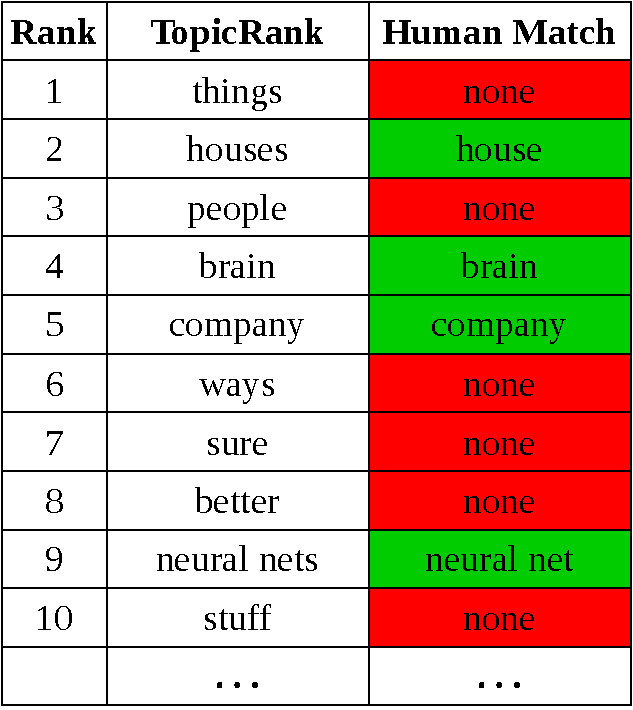
\includegraphics[width=0.5\textwidth]{topicRankEval.pdf}
    \caption{Top 10 \glspl{keyphrase} as determined by TopicRank and human matches where appropriate.}
    \label{fig: topicrank eval}
\end{figure}
We use TopicRank on our hand-annotated transcripts and compare its selected topic-phrases against human-annotated topic-phrases. If a given transcript has $N_{h}$ human annotated \glspl{keyphrase}, the top $N_{h}$ \glspl{keyphrase} as determined by the TopicRank algorithm are extracted. If a \gls{keyphrase} extracted by TopicRank or its plural/singular version is also found to be a \gls{keyphrase} by the human annotator, it is a match. On the 4 annotated transcripts, TopicRank achieves an accuracy (i.e. overlap with human \glspl{keyphrase})
\begin{equation}
    \text{accuracy} = 0.45 \pm 0.20.
    \label{eq: topic rank accuracy}
\end{equation}

\subsection{Limitations}
Fig. \ref{fig: topicrank eval} shows the top 10 highest ranked \glspl{keyphrase} and its human annotated counterpart if it exists. This illustrates two limitations of TopicRank:
\begin{enumerate}
    \item Abstract nouns such as ``things", ``people" or ``ways" are identified as topics even though they do not indicate a topic.
    \item Adjectives that are included as \gls{keyphrase} candidates, such as ``better" most often do not indicate a topic.
\end{enumerate}

% Put this as limitation in TopicRank
Another issue is that key-words are often not repeated but still understood as the topic. Consider the following \glspl{utterance}:

\begin{table}[h]
    \begin{tabular}{l|l}
    $u_1$     & \textit{Do you have any pets?}                    \\
    $u_2$     & \textit{Yeah I've got a cat.}                        \\
    \end{tabular}
\end{table}

The word ``pet" is not repeated  but from the context of the conversation it is clear that the topic is still ``pets". To improve the topic matching, we thus need to match semantically \textbf{similar} words instead of just matching equal words.
